\chapter{Problema 3}

\section{10594 - Data Flow}

En el laboratorio de IIUC, se requiere enviar una enorme cantidad de datos desde el servidor local hacia el terminal. La configuraci�n del laboratorio aun no esta lista. Requiere escribir un programa de ruteo para el mejor camino de datos. El problema es que todos los enlaces de la red tienen una capacidad fija y no puede fluir por ellos una cantidad mayor. Tambi�n toma una cierta cantidad de tiempo enviar una unidad de datos a trav�s del enlace. Para evitar las colisiones solo una unidad de datos puede viaja a la vez, por lo tanto, en un instante de tiempo no puede viajar en la red m�s de una unidad de datos en paralelo. Esto puede ser que consuma mucho tiempo pero asegura que no habr� colisiones. Cada nodo tiene suficiente capacidad de buffer de manera que los datos pueden ser temporalmente almacenados all�. La administraci�n de IIUC desea el menor tiempo posible para enviar todos los datos desde el servidor local hacia el final.

\begin{figure}[H]
\centering
\label{ejEnunciado_dataflow}
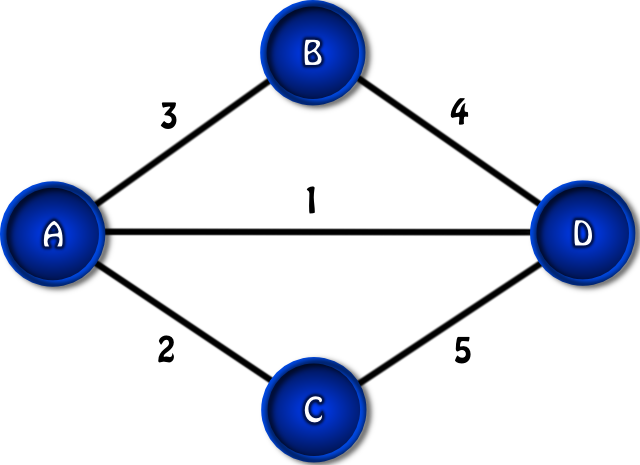
\includegraphics[scale=0.8]{./graficos/ej3/ejEnunciado.png}
\end{figure}

Por ejemplo, en esta red si alguien quiere enviar 20 unidades de datos desde A a D, enviar� 10 unidades de datos a trav�s del enlace AD y luego 10 unidades de datos a trav�s del enlace AB-BD, lo que tomar� 10+70=80 unidades de tiempo.

\textbf{Entrada:}

Cada input comienza con dos enteros positivos \textbf{N} ($2 \leq N \leq 100$), \textbf{M} ($1 \leq M \leq 5000$). En las siguientes l�neas siguen los links con su correspondiente tiempo de propagaci�n. Los links son bidireccionales y puede haber como m�ximo un link entre dos nodos de la red. En la siguiente l�nea habr� dos enteros positivos \textbf{D}, \textbf{K}, donde \textbf{D} es la cantidad de datos a ser transferida desde el 1er nodo hacia el \textbf{N}-�simo, y \textbf{K} es la capacidad de los enlaces. El input es terminado por EOF.

\textbf{Salida:}

Para cada test,  imprimir en una l�nea el m�nimo tiempo posible  para enviar todos los datos. Si no es posible enviar todos los datos, imprimir \"Impossible.\". El tiempo puede ser a lo sumo $10^{15}$.

\textbf{Url:}

\href{http://uva.onlinejudge.org/index.php?option=com_onlinejudge&Itemid=8&category=17&page=show_problem&problem=1535}{Problema de data flow}

\subsection{Modelo}

El modelo corresponde a un problema de flujo m�ximo de costo m�nimo, donde la red se representa mediante un grafo dirigido \textbf{G = (V, E)}, de forma tal que cada nodo $v_i \in$ \textbf{V} para $i = 1,2,...,N$ (el \textbf{N} del enunciado) representa un servidor en la red, y un eje $e = (v_i, v_j, w, f, c) \in$ \textbf{E} si hay un link entre los servidores representados por $v_i$ y $v_j$ que tiene un costo de w unidades de tiempo y contiene flujo f y capacidad c, con $f \leq c$. El grafo del modelo tendr� 2M ejes, siendo \textbf{M} el del enunciado.

\subsection{Soluci�n}

Dado el input construimos G y computamos Ford-Fulkerson y Bellman-Ford sobre �l.

El grafo residual no se calcula, sino que se realiza todo en G que tendr� ejes de costo positivo y ejes de costo negativo, de forma que cada link de $v_1$ a $v_2$ se representa mediante dos ejes: un eje $(v_1, v_2, w, f, c)$ y otro eje $(v_1, v_2, w, -f, c)$. Sin embargo durante la ejecuci�n de Bellman-Ford, consideramos que cuando el flujo de un eje es negativo, el mismo abarata el costo total (resta al costo total del camino) y si es positivo lo encarece (suma al costo total del camino).
\begin{itemize}
\item	Ford-Fulkerson: sirve para calcular el flujo m�ximo de una red. Necesita un G con ejes con capacidades c, un nodo fuente s y un sumidero t. El G es construido del input, y el s y t son dados (el nodo 1 y el nodo N respectivamente).

\item	Bellman-Ford: dado que en el problema existen ejes negativos, no podemos usar Dijkstra, por lo tanto optamos por usar Bellman-Ford para buscar caminos de aumento en el grafo residual (que est� dentro de nuestro G). Como en el grafo original los ejes tienen costo positivo, no se generan ciclos de costo negativo. Por lo tanto las precondiciones de Bellman-Ford se cumplen. Para poder pasar flujo por un eje se tiene que cumplir que $f < c$, por lo tanto al realizar Bellman-Ford solo tenemos en cuenta tales ejes como posibles candidatos a formar parte de un camino de aumento (pues tales ejes no pertenecen al grafo residual). Recibe dos par�metros: el nodo desde donde se calcula la menor distancia a todos los dem�s, y el grafo, y devuelve las distancias a todos los dem�s nodos. Lo ejecutamos entonces en cada paso de Ford-Fulkerson envi�ndole el grafo G y el nodo fuente s y luego aumentamos el flujo de los ejes del camino en c (la capacidad de los links) y restamos c al flujo de los ejes del camino en sentido contrario.
Este algoritmo efectivamente resuelve el problema, dado que por lo visto en clase, si cada camino de aumento que buscamos es de costo m�nimo respecto de los caminos de aumento disponibles, entonces el flujo resultante es de costo m�nimo.
\end{itemize}
\subsection{Detalles de implementaci�n}

Implementamos una clase \textbf{Red} que ser�a el grafo con ejes con costo y flujo. Dado el problema y nuestra soluci�n concluimos que todos los ejes tienen la misma capacidad, por lo tanto Red mantiene una variable para la capacidad de todos los ejes del grafo. Un eje est� compuesto de un nodo fuente y otro destino. Para los costos y flujos se mantienen dos matrices para poder consultar y asignar el costo y flujo de un eje en tiempo constante. Se mantiene adem�s una lista de adyacencias.

Se implement� una clase \textbf{ULLInt} (Unsigned Long Long Int) que representa los enteros y el valor infinito. Esto lo hicimos para poder inicializar las distancias a los dem�s nodos a infinito en el algoritmo de Bellman-Ford. Esta clase tiene implementados los operadores de suma y comparaci�n por mayor, de forma que $\infty > entero$ resulta verdadero, pero $\infty > \infty$ no.

Se implement� una clase \textbf{TestCase} que es la m�s importante, pues es la responsable de resolver el problema. Contiene la implementaci�n de Ford-Fulkerson (resolver) y Bellman-Ford (buscarCaminoMinimo).

\subsection{C�lculo de complejidad}

Bellman-Ford en peor caso es $O( NM )$ siendo \textbf{N} la cantidad de nodos y \textbf{M} la cantidad de ejes con un grafo implementado sobre listas de adyacencia.
Durante Ford-Fulkerson, cada vez que aumentamos el flujo lo hacemos en una magnitud c, siendo c la capacidad de los ejes, a excepci�n de la �ltima iteraci�n del algoritmo, que aumenta el flujo en $k mod c$, siendo k la cantidad de flujo a enviar. Por lo tanto Ford-Fulkerson itera $c/k$ veces.
Luego para finalizar calculamos el tiempo total empleado recorriendo todos los ejes del grafo y sumando $costo*flujo$ para aquellos ejes de $flujo > 0$. Esto tiene costo $O( M )$.
Concluimos que el algoritmo completo tiene complejidad $O( \frac{c*N*M}{k} + M ) \leq O( \frac{c*N*M}{k} )$
